\chapter{ОПРЕДЕЛЕНИЕ ТРЕБОВАНИЙ К ПРОГРАММНОЙ СРЕДЕ}



\section{Условия проведения олимпиады Ugra CTF}

Необходимо определить, какие из задач, связанных с проведением школьной олимпиады по защите информации Ugra CTF, подлежат автоматизации. В первую очередь, для этого необходимо разработать формальное описание этих задач. Существует ряд требований, который необходимо удовлетворить: внутренние и внешние.

Источников внутренних требований несколько. К ним относятся официальные нормативные документы: положение об олимпиаде и регламент её проведения. Регламент проведения олимпиады описывает следующие положения:

\begin{itemize}
\item порядок регистрации участников,
\item порядок проведения этапов олимпиады,
\item правила оформления и проверки работ,
\item порядок подведения итогов и др.
\end{itemize}

Эти требования составлены с учётом общих принципов проведения CTF-соревнований вида Jeopardy. Кроме того, поскольку требования внутренние, их допустимо видоизменять.

Ко внешним требованиям относится «Порядок проведения олимпиад школьников» \cite{Rosolymp}, документ, написанный РСОШ и утверждённый приказом Министерства образования и науки РФ. Этот документ, в частности, описывает общие положения и то, как должна проходить олимпиада. Большая часть требований РСОШ уже включена во внутренний регламент проведения олимпиады, и эти требования видоизменять нельзя.

Следует отметить, что перечисленные требования носит скорее юридический характер, и практически не устанавливает требования к технической инфраструктуре. Поэтому, их необходимо будет составить самостоятельно.

Кроме нормативно-правовых актов, регулирующих порядок проведения олимпиады и требования к участникам, существуют физические и технические ограничения, связанные с распределённо-очным форматом проведения олимпиады. Например, несмотря на сравнительную популярность CTF-соревнований, нельзя ожидать, что наблюдатели на площадках будут знакомы с особенностями этого формата и способны самостоятельно сконфигурировать подходящее сетевое и программное окружение для участников.

\subsection{Правила и порядок проведения олимпиады Ugra CTF}
\label{cha:the:rules-and-order}

Олимпиада состоит из двух этапов: отборочного (отбора, Ugra CTF Quals) и заключительного (финала, Ugra CTF School).

Отборочный этап проводится в дистанционном формате и состоит из двух зачётов. К участию в официальном зачёте допускаются обучающиеся школ и средне-специальных учебных организаций. Неофициальный зачёт открыт для всех желающих без ограничений, но не даёт права пройти в заключительный этап и имеет отдельную рейтинговую таблицу. Отборочный этап командный — в составе команды может быть от 1 до 5 человек.

Победители и призёры официального зачёта отборочного этапа олимпиады получают право на прохождение в заключительный этап. Заключительный этап, как отмечалось в § \ref{cha:analysis:ugractf}, проводится в распределённо-очном формате — участникам необходимо очно присутствовать на площадке. Заключительный этап индивидуальный — каждый участник решает задачи самостоятельно.

Оба этапа проходят по общем принципам. Зарегистрировавшиеся участники получают доступ к проверяющей системе — сайту олимпиады — на котором размещены задачи и форма для сдачи ответов. Ответом к каждому заданию является флаг — строка, удовлетворяющая регулярному выражению \texttt{ugra[A-Za-z0-9\_]\{2,\}}, например, \texttt{ugra\_ex4mpl3}.

\Define{Регулярное выражение}{текстовая строка особого формата, задающая конечный автомат для поиска определённой подстроки или подстрок в тексте}

В соответствии с принципами проведения CTF-соревнований в формате Jeopardy, за сданные в проверяющую систему флаги команда получает столько баллов, сколько стоило каждое задание. Побеждают участники, набравшие наибольшее количество баллов. При равенстве баллов побеждает участник, раньше решивший последнее задание.

По внутренним правилам олимпиады, на всех этапах запрещены следующие действия:
\begin{enumerate}
\item атака на инфраструктуру соревнований, к которой относятся, например, сервера, на которых размещена проверяющая система и задачи;
\item обмен условиями задач, если этот обмен не происходит между участниками одной команды во время отборочного этапа — в заключительном этапе этого исключения нет по причине индивидуального характера соревнований;
\item обмен флагами.
\end{enumerate}

Важно также соблюдать принцип равенства всех участников: никто не должен обладать преимуществом. Преимуществом можно считать как получение внешней помощи, например, путём публикации условий задач на интернет-форуме, так и ситуацию, в которой одной команде на решение было дано больше времени, чем другой — приём проверяющей системой флагов должен прекращаться одновременно для всех участников точно в момент окончания соревнований.

РСОШ требует предоставлять подробную отчётность об организации и проведении олимпиад, а также их результатах. В эту отчётность должны входить работы участников — в контексте CTF ими являются флаги: как верные, так и неверные.

\subsection{Подход к построению системы проведения испытаний}

Рассмотрим два подхода к проектированию архитектуры программных систем.

Первый — монолитный, когда все задачи выполняются в рамках одной большой неделимой системы. Авторы статьи «Проблемы реализации монолитных систем» \cite{Fomin21} предостерегают о недостатках такого подхода: «Поскольку любые развивающиеся [системы] рано или поздно начинают расти, необходимо периодически пересматривать архитектуру. На первых порах еще есть возможность контролировать процесс расширения монолитной архитектуры, но в определенной момент может оказаться, что для добавления совсем незначительной функциональности, нужно будет обновлять множество компонентов сразу». Эти проблемы особенно актуальны, поскольку правила олимпиады и требования к её проведению меняются из года в год под влиянием различных внешних факторов \cite{Olymp20} \cite{Olymp}, и система должна постоянно адаптироваться к этим изменениям — иными словами, постоянно развиваться.

Второй подход — модульный. При таком подходе реализуемая система есть комплекс из модулей — разделённых независимых подсистем, взаимодействующих между собой. Модульная система получится гибкой: её функциональность можно изменять, изменяя набор модулей, входящих в её состав. Это решение, на архитектурном уровне рассчитанное на расширяемость, которое в будущем может быть адаптировано и под различия правил отбора и финала, и под новые форматы и требования. К недостаткам такого подхода с технической точки зрения можно отнести необходимость разработки единого интерфейса, посредством которого должны взаимодействовать подсистемы \cite{Parnas85}, а с организационной — наличие нескольких независимых кодовых баз, поддерживать которые может оказаться непростой задачей \cite{Fomin21}.

\Define{Модуль системы}{независимая подсистема, взаимодействующая с другими компонентами системы}

Важно отметить, что требования к проведению отборочного этапа олимпиады есть подмножество требований к проведению заключительного этапа с точностью до малозначительных нюансов и определения сущности участника: как отмечалось выше, в первом случае это команда из нескольких человек, в другом — один человек. Такая вложенность согласуется с принципами абстракции при модульном подходе, поэтому в работе используется именно он.

Таким образом, проектирование системы должно быть сведено к разработке двух её модулей:
\begin{itemize}
\item система управления ходом испытания (материалами олимпиады, решениями и прочим),
\item система, предоставляющая участникам программную среду для прохождения испытания (и доступ к первой системе),
\end{itemize}
а также поиску способа интеграции этих двух модулей. Такое разделение позволяет единожды спроектировать систему, управляющую ходом соревнований любого формата и при необходимости подключать к ней вторую компоненту — программную среду.


\section{Система управления ходом испытания (борда)}

Контроль за ходом первых CTF-соревнований осуществлялся практически полностью вручную. Так, участники первых DEF CON CTF отправляли флаги оргкомитету в текстовом чате \cite{defcon}. Со временем стали появляться автоматизированные решения, которые автоматически генерировали флаги, размещали их в сервисах команд и принимали посылки участников по протоколу TCP — в числе первых предприняли меры автоматизации процесса проверки решений организаторы международных студенческих соревнований iCTF \cite{vigna2014:ictf}.

\Abbrev{TCP}{(англ. transmission control protocol) — сетевой протокол транспортного уровня, используемый для передачи данных с подтверждением получения}

Соревнования вида Jeopardy с самого начала были автоматизированы \cite{Kolegov08}. Это связано с относительно более тривиальным игровым процессом, чем в соревнованиях вида Attack-defense. Обычно участники получают доступ к веб-приложению, которое содержит условия задач, турнирную таблицу и форму для сдачи флага. Его принято называть \textit{бордой.}

\Define{Борда}{\textit{(англ. board, буквально «доска»)}~--- программная платформа для получения условий задач и сдачи флагов в CTF-соревнованиях вида Jeopardy}


\subsection{Требования к системе}

\subsubsection{Организационные требования к системе}
\label{cha:the:board:org}

Внутренний регламент проведения олимпиады и положение РСОШ предъявляют большое число требований к тому, каким образом участникам выдаются материалы олимпиады (задачи) и оцениваются работы.

\begin{enumerate}

\item
  Борда должна содержать все условия опубликованных задач. Допускается публикация новых задач после начала мероприятия и изменение условий уже опубликованных, если они содержат ошибки.

\item Борда должна обеспечивать контроль за временем начала и окончания олимпиады, не позволяя участникам получать очки за флаги, сданные вне этого времени.

\item Борда должна учитывать разных участников: предоставлять абстракцию для реализации их регистрации, различать участников официального и неофициального зачётов отборочного этапа.

\item По окончании испытания, на борде должны публиковаться предварительные результаты, причём, на отборочном этапе допускается публиковать предварительные результаты непосредственно во время мероприятия, динамически обновляя их.

\item
  Борда отвечает за проверку решений участников — валидацию флагов. Валидация должна осуществляться безошибочно, причём ответы участников, вне зависимости от их верности, необходимо фиксировать для отчётности. Приём решений должен начинаться и заканчиваться одновременно для всех участников вместе с, соответственно, началом и окончанием соревнований.

\item
  Желательно, чтобы в борде был предусмотрен механизм, позволяющий определять, самостоятельно ли участник получил флаг. Это позволит обеспечить более тщательный контроль за соблюдением пункта 20 положения РСОШ: «Во время проведения олимпиады участникам олимпиады запрещается иметь при себе средства связи, [...] и иные средства хранения и передачи информации, за исключением средств, разрешенных организатором олимпиады в условиях и требованиях по проведению олимпиады [...].» \cite{Rosolymp}.

\item Согласно внутреннему регламенту: «[...] участники могут задавать вопросы членам Жюри посредством Проверяющей системы» \cite{Olymp}.

\item Наконец, следует учесть, что CTF~--- творческий формат, поэтому структура и принципы могут меняться от игры к игры. Так, однажды оргкомитет олимпиады проводил экспериментальные соревнования в модифицированном варианте Jeopardy, [bank Bank] CTF \cite{Bankbank}. Эти соревнования были устроены в виде модельного теста на проникновение в корпоративную систему условного банка. Участникам были доступны не все задачи сразу, как это принято. Сперва игроку доступна лишь точка входа~--- сайт организации; по мере изучения системы открываются новые задачи, причём, какая именно задача откроется следующей, определяет древовидная структура.

\end{enumerate}

\subsubsection{Технические требования к системе}
\label{cha:the:board:tech}

Из организационных требований можно вывести ряд технических требований, которым должна удовлетворять борда.

\begin{enumerate}

\item
В первую очередь, к таким требованиям можно отнести устойчивость к высоким нагрузкам. В отличие от соревнований вида Attack-defense, где нагрузка команды атакуют друг друга (отношение «многие ко многим»), в Jeopardy участники взаимодействуют с централизованной игровой инфраструктурой организаторов (отношение «многие к одному»). Отказ в обслуживании со стороны игровой платформы категорически недопустим, поскольку он создаёт неравные условия для игроков: возможна ситуация, когда часть участников успеет получить условие задачи или сдать флаг, в то время как другая~--- нет.

Основные операции в платформе должны выполняться быстро и без существенных задержек. Желательно, чтобы система поддерживала многопоточную обработку пользовательских запросов там, где это возможно.

\item
Многопоточность, однако, зачастую приводит к неопределённости параллелизма~--- ошибке проектирования многопоточной системы или приложения, при которой работа системы или приложения зависит от того, в каком порядке выполняются части кода. Эта неопределённость может послужить причиной ошибок: например, к двойному начислению баллов или списанию некорректной суммы баллов при взятии подсказок.

\Define{Неопределённость параллелизма}{ошибка проектирования многопоточной системы или приложения, при которой работа системы или приложения зависит от того, в каком порядке выполняются части кода}

\item
Тот факт, что соревнования~--- по защите информации, накладывают повышенные требования к безопасности платформы. Несмотря на то, что правилами Ugra CTF запрещены атаки на инфраструктуру, непосредственно не относящуюся к игровым задачам, попытки вывести её из строя всё равно предпринимаются. Система должна быть устойчивой к наиболее распространённым веб-уязвимостям (например, связанным с обработкой запросов или контролем пользовательских сессий), а также вести аудит всех событий для своевременного обнаружения оргкомитетом новых угроз.
\end{enumerate}

\subsection{Материалы олимпиады (задачи)}

\subsubsection{Описание и структура задачи}

Материалы олимпиады — это набор задач, которые участники решают. С точки зрения информационной модели системы, задачу можно представить как структурированный объект, включающий в себя следующие данные:

\begin{enumerate}
\item название;
\item стоимость в баллах;
\item игровая категория;
\item текстовое условие;
\item вложения и внешние ссылки (необязательно);
\item флаг — ответ на задачу.
\end{enumerate}

\subsubsection{Классификация задач}
\label{cha:the:classes}

Тематика задач не ограничивается ни одним из требований, рассмотренных выше. Её принято классифицировать согласно категориям, данным в § \ref{cha:analysis:Jeopardy}, но эта классификация мало чем полезна с точки зрения разработки борды и в первую очередь нацелена на участников, как отмечалось в вышеупомянутом параграфе.

Удобнее ввести другой способ классификации задач: по типу связанных с ней ресурсов. Например, если задача связана с анализом и эксплуатации уязвимостей веб-приложения, то необходимо обеспечить доступ участника к нему, предоставив ссылку на запущенный экземпляр этого приложения. Или, если задача связана с криптографическим анализом, в её вложениях должен содержаться файл с шифртекстом. Способ представления задачи на борде и процедура публикации задачи, а следовательно, и новые организационные обстоятельства, во многом зависит от связанных с ней ресурсов.

Рассмотрим классификацию задач относительно типов связанных с ними ресурсов. При изучении корпуса задач Ugra CTF за 2016---2021 годы было определено четыре типа ресурсов (таблица \ref{tab:tasks}). В таблице приведены классы задач, типы связанного ресурса, организационно-технические задачи, которые необходимо решить, чтобы ресурс был доступен участникам, и данные о задаче в борде, на которые влияет ресурс.

\begin{longtable}{|p{2.9cm}|p{0.34\textwidth}|p{0.22\textwidth}|p{0.15\textwidth}|}
  \caption{Классификация задач по типам связанных с ними ресурсов.}
  \label{tab:tasks}
  \\ \hline
  \textbf{Класс задач} & \textbf{Тип связанного~ресурса} & \textbf{Что необходимо} & \textbf{Зависимые данные}
  \\ \hline \endhead
  сетевые & приложение с доступом по сетевому протоколу & запущенный сервер приложения & ссылка в~описании
  \\ \hline
  динамические & программно генерируемое вложение & запущенная единожды программа-генератор & вложения
  \\ \hline
  статические & созданное вручную вложение &~--- & вложения
  \\ \hline %
\end{longtable}

\Abbrev{IP}{Internet Protocol}
\Abbrev{URL}{Uniform Resource Locator}

\Define{Сетевая разведка \textit{(англ. OSINT, open-source intelligence)}}{поиск информации в открытых источниках}

\subsubsection{Процесс публикации задач}
\label{cha:the:decl-imper}

\begin{figure}[h!]
  \centering
  \includegraphics[width=\textwidth]{inc/svg/downtimes-before}
  \caption{Статистика доступности ресурсов задач. Данные оргкомитета.}
  \label{fig:downtimes-before}
\end{figure}

Опыт проведения соревнований в предыдущие годы показал, что авторы наиболее склонны совершать ошибки не сколько при составлении задач, сколько при их публикации. Публикация задач — монотонный, однообразный процесс, влияние человеческого фактора на который крайне необходимо свести к минимуму. Недоступность — пусть и кратковременная — хотя бы одного ресурса приводит к неравенству участников: возможность решить задачу в конкретный момент начинает зависеть от случайности.

На рисунке \ref{fig:downtimes-before} показано, что на соревнованиях Ugra CTF за 2018---2021 годы в среднем около $9\%$ от общего времени проведения испытания был недоступен хотя бы один ресурс. То есть при ручной публикации ресурсов задач ожидается, что на заключительном этапе олимпиады, продолжительность которого составляет 5 часов, 27 минут времени участников будет потрачено на ожидание устранения неисправностей.

Публикацию ресурсов задач можно автоматизировать, что должно положительно сказаться на их доступности. Изучим, как разрабатываются и публикуются задачи, а также связанные с ними ресурсы.

\FloatBarrier

Тривиален процесс для задач статического класса. Автор разрабатывает задачу, заполняет структурированные данные о ней и публикует её на борде. При необходимости разрабатываются вложения.

Необходимость в задачах динамического класса обуславливается тем, что не всегда вложения разумно создавать, используя ручной труд. Так, на отборочном этапе 2019 года участникам предлагалась разгадать шифр, вдохновлённый внутренним устройством электрической печатной машинки IBM Selectric \cite{Selectric}. Для этого во вложении к этой задачи был дан файл~--- объёмная модель конструктивной детали машинки. Создание модели было автоматизировано: автор задачи составил программу — генератор нужных моделей с разными параметрами.

% consider onionion from ugractf19

Наконец, есть класс сетевых задач. Ресурсы, связанные с такими задачами — это веб-приложения или сервисы, взаимодействующие посредством других протоколов — причём, самых разных: например, при сетевой задаче может быть развёрнута виртуальная машина, к которой необходимо получить доступ. Особенность этого класса задач заключается в наличии программы-сервера, которая должна быть доступна по конкретному адресу на протяжении всего испытания.

Чтобы опубликовать ресурсы такой задачи, необходимо, как минимум, выполнить большое количество действий, связанных с сетевым и системным администрированием, что на практике оказывается проблематичным для оргкомитета в условиях ограниченного времени на подготовку к олимпиаде и постоянно меняющимся условиям их проведения: разные сервера, разные домены соревнований, задачи, условия которых могут быть изменены «на ходу», ошибки технического характера и т.д. Именно задачи сетевого класса наиболее часто оказываются недоступными для участников, поэтому автоматизировать их публикацию наиболее важно.

Чтобы автоматизировать процесс публикации задач, необходимо разработать соответствующую компоненту борды. Для решения подобных вопросов в программировании существуют две парадигмы: императивная и декларативная \cite{Cioni88}.

В императивной парадигме программист определяет, \textit{как} можно решить проблему, т.е. какая последовательность действий позволит достичь требуемого результата, при этом, как правило, описание самого результата остаётся «за кадром». В то же время, в рамках декларативной парадигмы говорится только о результате, который программа должна вычислить, т.е. какова связь между входными и выходными данными, и при этом не уточняется, как компьютер будет его достигать.

Эти парадигмы полностью противоположны по своей сути, однако, это не означает, что использование одной парадигмы исключает использование другой. Рассмотрим этот вопрос на абстрактном примере публикации задачи об условном веб-приложении.

Первый подход — императивный. Описание процесса публикации сводится к разработке алгоритма. То есть, автор задачи, кроме ресурса этой задачи, напишет также и программу, при запуске которой выполнятся, например, следующие действия:

\begin{enumerate}
\label{enum:netalgo}
\item разместить программную часть ресурса на сервере испытаний;
\item установить все зависимости, необходимые для запуска программной части ресурса;
\item выделить адрес (IP либо URL) для доступа к программе ресурса по сети;
\item создать системный сервис, запускающий программную часть ресурса и перезапускающий его в случае критической ошибки;
\item изменить конфигурацию межсетевого экрана;
\item добавить ссылку на ресурс в описание задачи;
\item проверить доступности сервиса из игровой сети;
\item до окончания соревнований каждую минуту повторять предпоследний шаг.
\end{enumerate}

В таком случае, борде необходимо будет лишь выполнить эту программу, и задача окажется опубликованной. Проблема автоматизации решена.

Второй подход — декларативный. Описание процесса публикации сводится к описанию результата. Автор задачи опишет её, например так:

\textit{«Публикация задачи — это публикация одного ресурса. Ресурс — это веб-приложение на языке [...], доступное по адресу [...], порту [...], файлы которого находятся в каталоге [...] на сервере [...]».}

В этом случае, борде необходимо будет перевести описание результата в нужную последовательность действий самостоятельно — иными словами, автоматизирована будет не только публикация задачи, но и формирование \textit{алгоритма её публикации.}

Это наиболее желаемый подход, поскольку он избавляет составителей задач от необходимости составления алгоритмов вручную~--- почти все ошибки, возникающие при публикации задач, приводят к их недоступности. Важно, чтобы генерируемые автоматически алгоритмы публикации задач были корректными. Возможность гарантировать, что задача будет опубликована корректно, и есть основное преимущество декларативного подхода перед императивным. Однако, реализовать такую компоненту генерации алгоритмов публикации задач, которая была бы способна разработать алгоритм для произвольной задачи невозможно.

Получившаяся при таком подходе компонента генерации алгоритмов публикации задач должна включать в себя формальный язык, которым описываются задачи (позволяющий выражать факты, подобные примеру в кавычках выше), а также множество отношений между высказываниями на этом языке. То есть, по определению являться формальной системой \cite{Vereshen08-3}. Известно, что любая формальная система может быть либо неадекватной (порождать некорректные результаты), либо неполной (порождать не все корректные результаты) \cite{Vereshen08-3}. К тому же, проверка адекватности автоматически созданного алгоритма невозможна без непосредственного выполнения этого алгоритма — это следует из проблемы остановки, сформулированной А. Тьюрингом \cite{Turing37}. Раз существует вероятность получить в рамках компоненты либо некорректный алгоритм, либо такой алгоритм, который не выполнится никогда, и проверить это невозможно, то компонента генерации алгоритмов публикации задач должна быть неполной — содержать ограничения.

Таким образом, разработать полностью автоматическую систему публикации задач можно лишь совместив императивный и декларативный подходы так, что борда будет:

\begin{enumerate}
\item генерировать алгоритм публикации и выполнять его для некоторого узкого множества задач, выведенного из классификации задач из § \ref{cha:the:classes};
\item предоставлять автору возможность предоставления вручную разработанного алгоритма для остальных задач (и требовать ручной проверки результата).
\end{enumerate}

\subsubsection{Проверка решений}

Проверка решений участника тривиальна: борда должна принять его посылку и сопоставить её значение с каким-то флагом одной из опубликованных задач. Если сопоставить значение не удаётся, решение участника неверное.

Организационными требованиями к проведению олимпиады диктуется необходимость сохранять все посылки участника вне зависимости от их правильности. Кроме того, важно проверять не только правильность, но и самостоятельность решения задач.

Если отказаться от использования задач статического класса в пользу задач динамического класса, то возможна генерация задачи «по вариантам»: с общим принципом решения, но уникальным для каждого участника ответом. В этом случае любая попытка недобросовестной сдачи участником флага, ему не предназначенного, автоматически считается неверной.

Это достижимо путём обязательной генерации по экземпляру задачи на каждого участника с добавлением во флаг каждого экземпляра значения хеш-функции от некоторого уникального идентификатора участника. Будем называть такое значение \textit{суффиксом варианта.} Хеш-функция~--- это функция, отображающая входное слово конечной длины в конечном алфавите в слово заданной, обычно фиксированной длины \cite{Cryptodict}. Результат работы хеш-функции должен обладать фиксированной длиной, чтобы общая длина флагов, от которой может напрямую зависеть сложность решения задачи, осталась неизменной для всех участников. Для исключения возможности участников генерировать флаги разных вариантов самостоятельно, хеш-функция должна быть криптографической и задаваться ключом, то есть задачи поиска коллизий и прообразов её значений должны быть вычислительно трудными \cite{Cryptodict}, а её применение~--- невозможным без знания ключа.

Создание суффикса варианта должно осуществляться на стороне задачи, а не борды, поскольку специфика задач может накладывать ограничения на длину и алфавит флага. Это, например, распространено в задачах, связанных с криптографией и стеганографией. К тому же это позволит легко изменять ключ, которым задаётся хеш-функция от задачи к задачи.

Таким образом, для генерации задач «по вариантам», необходимо предусмотреть в борде функциональность, обеспечивающую каждого участника внутренним уникальным идентификатором, необходимым для вычисления суффикса варианта, а также программный интерфейс между бордой и генераторами задач для передачи между ними, с одной стороны, упомянутого идентификатора, с другой — готовых флагов.

Осталось рассмотреть внедрение аналогичного механизма защиты для задач сетевого класса. Поскольку при решении таких задач игроки взаимодействуют с компьютерными программами, то, в целях экономии вычислительных ресурсов и сетевого адресного пространства оргкомитета, следует избегать генерации и запуска по уникальному экземпляру такой программы на каждого участника. Вместо этого рациональнее запускать один экземпляр, способный и генерировать суффиксы варианта, и получать идентификаторы, но уже не от борды, а от игрока~--- динамически. Например, если есть веб-приложение, в котором страницы имеют адреса вида: \texttt{http://example.ugractf.ru/page/}, то после реализации в нём описанной логики, адреса дополнятся префиксом: \texttt{http://example.ugractf.ru/}[уникальный идентификатор участника]\texttt{/page/}, чтобы передать приложению данные для генерации флага.

Стоит учесть, что если участнику известен свой уникальный идентификатор, и он не изменяется от задания к заданию, то это увеличивает шансы участника на успешный криптографический анализ процедуры создания суффикса вариантов и, следовательно, на обход механизма защиты. Существенно затруднить анализ можно, заменив константный идентификатор косвенным. Косвенный идентификатор участника — это значение хеш-функции от единственного уникального идентификатора, который хранится в борде, причём для каждой задачи используется хеш-функция, задаваемая своим ключом, так же, как и при создании суффикса вариантов. Тогда с точки зрения игрока и его идентификатор, и суффикс флага будут похожи на непредсказуемые случайные значения, логику в получении которых сложно предсказать, даже если в качестве прямого уникального идентификатора используется, например, порядковый номер участника или адрес его электронной почты.


\Define{Хеш-функция}{функция, отображающая входное слово конечной длины в конечном алфавите в слово заданной, обычно фиксированной длины}
\Define{Коллизия}{для хеш-функции $h$ — такая пара значений $x, y, x \ne y$ её аргумента, что $h(x) = h(y)$}
\Define{Уникальный (прямой) идентификатор участника}{данные, позволяющие однозначно определить участника в среде для проведения испытаний}
\Define{Косвенный идентификатор участника}{значение хеш-функции от единственного уникального идентификатора, который хранится в борде}

\subsection{Интерфейсы модуля}

Интерфейс — совокупность средств, методов и правил взаимодействия между элементами системы \cite{Nostroi}. Модуль контроля за ходом испытаний должен взаимодействовать с другими компонентами посредством программных интерфейсов, а также с пользователями: участниками и организаторами.

\Define{Интерфейс}{совокупность средств, методов и правил взаимодействия между элементами системы}

Участникам борда должна предоставлять пользовательский интерфейс, из которого доступны:
\begin{enumerate}
\item список опубликованных задач;
\item описание каждой задачи, включая:
  \begin{enumerate}
  \item \textit{метаданные:} название, категорию и стоимость,
  \item текст условия,
  \item вложения (если имеются);
  \end{enumerate}
\item поле для ввода флага,
\item форма для связи с оргкомитетом (для распределённо-очного этапа);
\item сведения об участнике, включая:
  \begin{enumerate}
  \item имя, псевдоним или название команды,
  \item количество набранных баллов;
  \end{enumerate}
\end{enumerate}

Интерфейс участника должен быть доступен только авторизованным пользователям и поддерживать разные механизмы аутентификации, поскольку они отличаются на разных этапах соревнований Ugra CTF:

\begin{itemize}
\item
  Участники отборочного этапа получают от «Юрта» электронное письмо со ссылкой для входа в проверяющую систему, содержащую токен — псевдослучайную последовательность символов с достаточной для надёжной аутентификации энтропией.
\item
  Участникам заключительного этапа запрещено использовать средства связи, поэтому данные для входа они должны получать на бумажном носителе: в таком случае, чтобы не заставлять игроков перепечатывать с листа длинный токен, желательно предусмотреть возможность аутентификации с использованием пары «логин-пароль».
\end{itemize}

\Define{Токен}{пседвослучайная последовательность символов с достаточной для надёжной аутентификации энтропией}
\Abbrev{ИС}{информационная система}

Регистрация участников происходит посредством отдельной и уже разработанной оргкомитетом информационной системы «Юрт», поэтому в борде необходим программный интерфейс, связывающий эти две системы и позволяющий выгружать данные о зарегистрированных пользователях.

Организаторам должна предоставляться возможность управлять конфигурацией борды, управлять участниками, публиковать, удалять и редактировать задачи. Пользовательский интерфейс для организаторов желателен, но разрабатывать его не требуется, поскольку предполагается, что они имеют прямой доступ и к базе данных борды, и к её программному коду, и этого доступа достаточно, чтобы взаимодействовать с системой.


\subsection{Анализ аналогичных существующих систем}

Существует множество программных продуктов, позволяющих проводить Jeopardy -- CTF-соревнования: организаторам необходимо лишь собрать участников, разработать задания и загрузить их на готовую платформу.

\begin{figure}[h!]
  \centering
  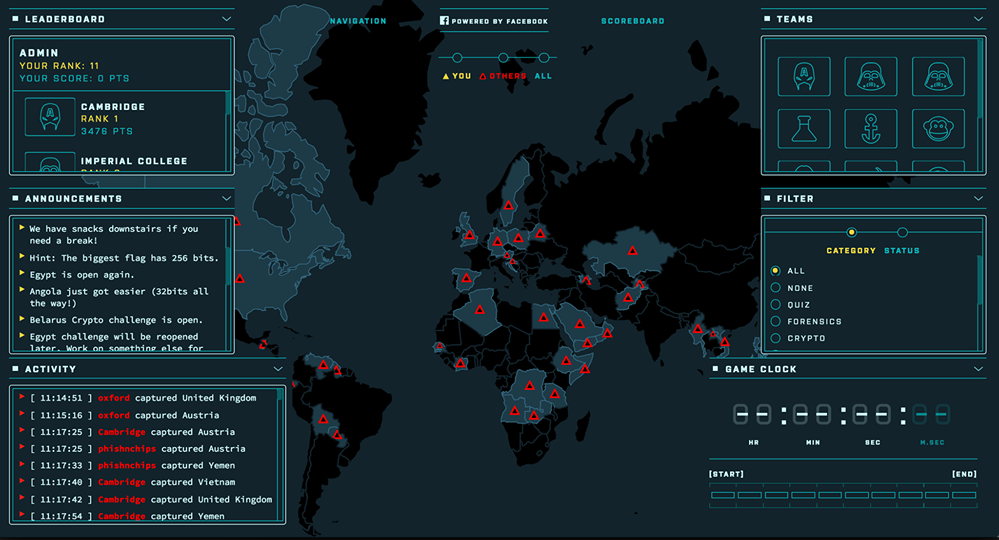
\includegraphics[width=0.9\textwidth]{inc/img/fbctf}\\
  \caption{Главная страница соревнования на платформе FBCTF.}
  \label{fig:fbctf}
\end{figure}

Проведём краткий анализ функциональности и особенностей реализации наиболее популярных готовых проверяющих систем для Jeopardy CTF. Выборка состоит из трёх систем, наиболее популярных на ресурсе GitHub \cite{GithubCTFTag} по тегу «ctf board» (yatb \cite{yatb}, picoCTF \cite{picoctf}, mellivora \cite{mellivora}), а также трёх систем, которые используются для проведения наиболее популярных международных соревнований по статистике агрератора CTFTime.org \cite{CTFTime} (Google kCTF \cite{kctf}, FBCTF, ctfd \cite{ctfd} (таблица \ref{tab:comp}).

\begin{longtable}{|p{5cm}|p{1cm}|p{1cm}|p{1.5cm}|p{1.5cm}|p{1.8cm}|p{2cm}|}
  \caption{Сравнительный анализ наиболее популярных платформ для Jeopardy CTF}
  \label{tab:comp}
  \\ \hline
  \textbf{Платформы / критерий~сравнения} & \textbf{ctfd} & \textbf{yatb} & \textbf{kCTF} & \textbf{FBCTF} & \textbf{picoCTF} & \textbf{mellivora}
  \\ \hline \endhead

  Лицензия & комм. & своб. & своб. & огран. & своб. & своб.
  \\ \hline
  Изменение материалов & + & + & + & + & + & +
  \\ \hline
  Валидация флагов     & + & + & + & + & + & +
  \\ \hline
  Хранение всех посылок участников & + & + & - & - & - & +
  \\ \hline
  Проверка уникальности решения & - & - & - & - & - & -
  \\ \hline
  Устойчивость к высоким нагрузкам  & - & + & + & + & + & -
  \\ \hline
  Поддержка многопоточности & + & + & + & + & - & -
  \\ \hline
  Логирование событий & + & + & - & + & - & -
  \\ \hline
  Поддержка произвольных форматов игры & - & - & - & - & - & -
  \\ \hline

\end{longtable}

Каждая из этих платформ, кроме Google kCTF~--- это монолитное приложение с веб-интерфейсом, встроенной системой регистрации, аутентификации и авторизации пользователей. Платформа Google kCTF обладает модульной микросервисной архитектурой: каждая её функциональная компонента представляет собой отдельную программу; взаимодействие между компонентами осуществляется через сетевые протоколы.

Ни одна система не удовлетворяет одновременно всем необходимым требованиям, предъявляемым к борде для проведения испытаний Ugra CTF, описанных в предыдущих разделах (табл. 2.1).

Поддержка декларативного описания материалов испытаний (задач) также не предусмотрена ни одним из решений. Более того, некоторые платформы, например, ctfd, вообще поддерживают лишь добавление материалов на платформу только посредством графического интерфейса (рисунок \ref{fig:ctfd}), который позволяет указать метаданные задачи лишь вручную~--- причём, по одной за раз, что затрудняет процесс подготовки к соревнованиям. Следует отметить, что именно эта платформа использовалась оргкомитетом Ugra CTF в ранние годы, и опыт работы с ней и привёл организаторов к необходимости разработки своего решения.

\begin{figure}[h!]
  \centering
  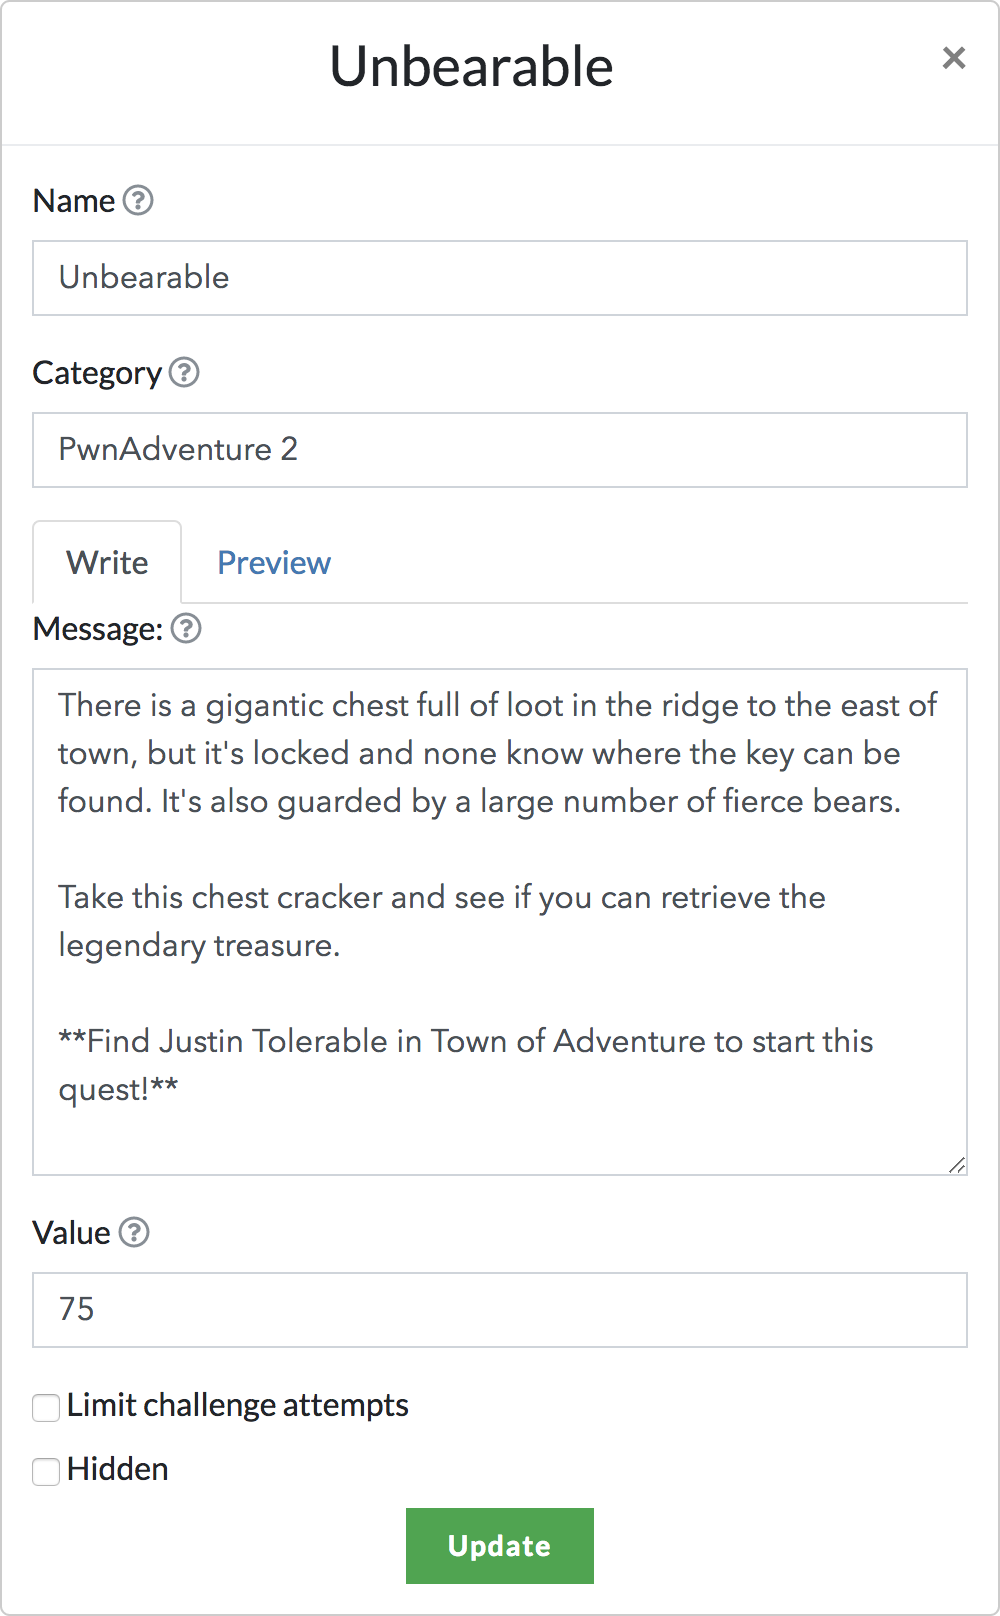
\includegraphics[width=0.33\textwidth]{inc/img/ctfd}\\
  \caption{Редактирование метаданных задачи на платформе ctfd.}
  \label{fig:ctfd}
\end{figure}


\FloatBarrier



\section{Система, предоставляющая участникам программную среду для решения задач}

Данный модуль необходим в случаях, когда испытания проводятся в распределённо-очном формате. На сегодняшний день, как отмечалось в § \ref{cha:the:rules-and-order} такой формат используется при проведении заключительного этапа Ugra CTF School.

\subsection{Предпосылки для разработки}

Чтобы проводить испытания в области защиты информации в формате CTF, участнику нужен компьютер. Компьютеры предоставляются участниками централизованно: это входит в обязанности площадок, на которых проводятся олимпиада. Это связано, в первую очередь, с тем, что положением проведения олимпиады Ugra CTF School \cite{Olymp} устанавливается запрет на использование участниками любых технических средств, включая собственные компьютеры.

Решение CTF-задач может потребовать от участников выполнения на предоставленных площадками компьютерах (рабочих станциях) самых разных действий, например, установки дополнительного программного обеспечения. Здесь возникает проблема.

В современных операционных системах для выполнения многих действий, связанных с изменением конфигурации ОС, требуется привилегированный доступ («права администратора» в ОС Windows, «права суперпользователя» в UNIX-подобных ОС). Произвольное изменение участниками конфигурации ОС компьютеров, предоставляемых площадкой, нежелательно, поскольку проведение олимпиады~--- далеко не основная задача, для которой они используются. К тому же, участник с привилегированным доступом вполне способен на совершение деструктивных действий, которые могут привести к утрате работоспособности его рабочей станции и вынудят наблюдателей затратить ресурсы на исправление возникших проблем. В связи с этим, оргкомитету желательно иметь возможность гарантировать, что ни компьютеры организации, предоставляющей площадку, ни данные, на нём хранящиеся, не должны пострадать от действий участников.

С другой стороны, имеющаяся на компьютерах ОС может быть либо устаревшей, либо малознакомой участнику~--- это отрицательно повлияет на его продуктивность в ходе испытаний.

Наконец, одна из задач, которую в своей совокупности должна решать среда для проведения дистанционных испытаний~--- контроль соблюдения правил испытаний. Это достигается путём внедрения автоматизированных инструментов для наблюдения за действиями участника~--- то, что называется прокторингом \textit{(англ. proctor~--- наблюдатель за ходом экзамена)}. Это, в свою очередь, требует возможности сопоставлять рабочие станции и личности участников.

\Define{Прокторинг}{процесс (автоматизированного) наблюдения за действиями участника испытаний}

То есть, необходимо предоставить участникам такую среду, которая:
\begin{itemize}
\item
  позволит участникам пользоваться предоставленным компьютером для решения игровых задач без дополнительных сложностей;
\item
  позволит организатором осуществлять контроль за действиями участников;
\item
  не потребует внесения необратимых изменений в рабочих компьютеров;
\item
  должна устанавливаться на компьютеры площадки при минимальном участии наблюдателей.
\end{itemize}


\subsection{Установка и инициализация среды}

Чтобы исключить зависимость среды от ОС, уже установленной на компьютеры площадки,  предоставление среды для решения задач должно включать в себя предоставление собственной ОС. Это позволяет также полностью исключить использование встроенного накопителя рабочих станций~--- современные компьютеры поддерживают загрузку ОС со внешнего накопителя \cite{USBBoot}. На этом же внешнем накопителе рационально разместить и остальные компоненты среды.

Инициализация среды должна проходить в автоматическом режиме. Этот процесс включает в себя обнаружение периферийных устройств рабочей станции (клавиатуры, мыши, монитора), а также конфигурацию графического и сетевого адаптера.

Прогресс инициализации должен сопровождаться графической либо текстовой индикацией прогресса, которая, в случае возникновения неполадки сопровождается информацией о причине неполадки и возможном пути её устранения. При этом, в случае, если на момент возникновения неполадки среда уже имеет доступ в интернет, необходимо предусмотреть возможность удалённого доступа к ней для организаторов, а также наличие централизованного пользовательского интерфейса, который отображал бы актуальное состояние всех рабочих станций.

Инициализация считается завершённой, когда компьютер готов к использованию участником. Индикация прогресса инициализации должна завершаться выводом на экран сведений об участнике, для которого предназначена конкретная рабочая станция.

Чтобы исключить возможность участника или наблюдателя повлиять на работу компонентов среды, необходимо исключить возможность модифицировать содержимое внешнего накопителя, на котором хранится среда, а сами данные, записанные на нём считать эталонными. Это сделает невозможным попытки обхода, например, механизмов прокторинга.



\subsection{Использование технологий виртуализации в среде}

Как отмечалось выше, для решения задач в ходе испытаний участник должен обладать привилегиями суперпользователя (администратора). Предоставлять такой доступ непосредственно к ОС, инициализирующей среду, нерационально. Обладая такими привилегиями, участник может, во-первых, обойти любой механизм защиты от изменения содержимого внешнего накопителя, во-вторых, нарушить работоспособность своей рабочей станции. Подобные нарушения не всегда исправимы: например, в 2016 году оказалось, что что операция рекурсивного удаления всех файлов на диске компьютера под управлением ОС Linux в ряде случаев затрагивала переменные UEFI \textit{(англ. universal extensible firmware interface~--- интерфейс между ОС и аппаратным обеспечением компьютера),} что приводило необратимому к выводу из строя материнской платы \cite{EFIrm}.

Вместо этого среда может предоставлять участнику виртуальную машину поверх основной ОС. Виртуальная машина (ВМ) — это программа, работающая на оборудовании физической машины (называемой \textit{хостом),} которая предоставляет изолированную среду с собственной \textit{гостевой ОС}, отделенными от ОС хоста и других ВМ этой хост-системы \cite{HPEVM}.
Использование ВМ в рамках среды для проведения испытаний обладает целым рядом преимуществ.

Во-первых, при корректной конфигурации, ВМ полностью разграничивает гостевую ОС и ОС хоста, что позволяет выдать участнику право совершать любые действия в виртуальной машине без риска нарушить функционирование среды ни на программном, ни на аппаратном уровне.

Во-вторых, некоторые ВМ поддерживают т.н. \textit{контрольные точки \cite{VMrollback}.} Состояние ВМ в конкретный момент времени, вплоть до значений регистров процессора, можно сохранить, создав такую контрольную точку, чтобы в будущем иметь возможность легко вернуться к нему. Это позволяет ставить эксперименты: участник, например, может запустить непроверенную программу, создав перед этим контрольную точку, и, в случае неуспеха, легко откатиться до неё при минимальных временных затратах.

Наконец, внутри ВМ можно использовать любую ОС, совместимую с аппаратной архитектурой хоста. Выбор ОС не зависит от выбора ОС хоста, никак не влияет на устройство остальной среды проведения испытаний, и определяется лишь образом~--- файлом, с которого «загружается» ВМ.

К недостаткам использования ВМ можно отнести повышенные требования к вычислительным ресурсам компьютера. В современных процессорах, однако, зачастую реализовано аппаратное ускорение виртуализации, позволяющая выполнять инструкции ВМ практически без потери производительности, а также предоставлять гостевой ОС прямой доступ в устройствам ввода-вывода без использования для этого программных абстракций \cite{VMWarex86}. В 2021 году на всех площадках проведения Ugra CTF были компьютеры с поддержкой этой технологии, что позволяет сделать вывод о её распространённости и внести наличие аппаратного ускорения виртуализации в перечень организационно-технических требований к оборудованию площадок.



\subsection{Выбор операционных систем}

Необходимо определить, на базе каких ОС должна функционировать сама среда (базовая ОС) и виртуальная машина, предоставляемая участнику (гостевая ОС). Установим ряд требований к этим ОС.

Прежде чем описывать технические требования, обратим внимание на законодательные аспекты. Программы для электронно-вычислительных машин (ЭВМ), включая ОС, охраняются авторским правом в соответствии со статьёй 1261 Гражданского кодекса Российской Федерации (ГК РФ) \cite{GK1261}. Следовательно, выбранные ОС должны распространяться по лицензии, позволяющей вносить изменения в их программный код и распространять модифицированные копии, обеспечивая возможность интеграции их в единую программную среду для проведения испытаний.

\Abbrev{ЭВМ}{электронно-вычислительная машина}
\Abbrev{ГК РФ}{Гражданский кодекс Российской Федерации}

Таким требованиям удовлетворяет так называемое свободное программное обеспечение~--- программы с лицензией, предоставляющей пользователю четыре свободы, сформулированные Фондом свободного программного обеспечения \textit{(англ. FSF~--- Free software foundation) \cite{GNUfree}:}
\begin{enumerate}
\item свобода запускать программу в любых целях;
\item свобода изучать работу программы и адаптировать её под различные нужды (доступ к исходным текстам ПО является необходимым условием почти любой свободной лицензии);
\item свобода распространять копии ПО;
\item свобода улучшать программу и публиковать эти улучшения.
\end{enumerate}



\subsubsection{Базовая операционная система~--- NixOS}

Базовая ОС должна:

\begin{enumerate}
\item
  обладать поддержкой разнообразного аппаратного обеспечения, поскольку конфигурация компьютеров на площадке неизвестна;
\item
  поддерживать работу в режиме \textit{Live USB (англ. дословно «живой USB-накопитель»)}~--- неперсистентной загрузки со внешнего носителя без установки на внутренний накопитель компьютера;
\item
  обладать системой разграничения прав (см. \ref{cha:the:init});
\item
  поддерживать технологии виртуализации;
\item
  быть легко модифицируемой, причём желательно, чтобы можно было создавать свои загрузочные образы с заранее определённой произвольной конфигурацией.
\end{enumerate}

Всем этим требованиям удовлетворяет ОС NixOS, дистрибутив ОС Linux, основанный на базе функционального пакетного менеджера Nix. В числе заявленных разработчиками возможностей стоит отдельно отметить наиболее важную для разработки среды: декларативную модель конфигурации системы \cite{NixOS}.

\Define{Пакет (в пакетном менеджере)}{особый архив, который содержит файлы (исходные коды либо исполняемые файлы) того или иного компонента ОС, а также метаданные, определяющие способ его установки в систему.}

Все компоненты NixOS являются пакетами~--- и ядро, и приложения, и системные модули. Пакет~--- это особый архив, который содержит файлы (исходные коды либо исполняемые файлы) того или иного компонента ОС, а также метаданные, определяющие способ его установки в систему. Эти пакеты управляются пакетным менеджером Nix \cite{Nixpkg}, а их описание составляется на специальном языке, который также называется Nix \cite{Nixlang}. Принцип «всё~--- это пакет» абсолютен:  каждый конкретный экземпляр NixOS, в конечном счёте, также является пакетом, сборка которого аналогичным образом описывается на языке Nix.

Рассмотрим полную конфигурацию минимального по функциональности экземпляра NixOS:

\begin{lstlisting}[caption={Минимальный пример конфигурации NixOS на языке Nix}]
{
  boot.loader.grub.device = "/dev/sda";  # определение загрузочного диска
  fileSystems."/".device = "/dev/sda1";  # ...и корня файловой системы
  services.sshd.enable = true; # включение удалённого доступа по SSH
}
\end{lstlisting}

Как видно, описанию на языке Nix подлежат абсолютно все аспекты ОС, включая как набор предустановленного ПО, так и низкоуровневые детали конфигурации, такие, как способ загрузки с диска~--- это всё можно переопределить самостоятельно, разработав свою собственную версию ОС, удовлетворяющую любым нуждам.

Важно отметить, что пакетным менеджером Nix предоставляются гарантии воспроизведения конфигурации в любом аппаратном контексте выполнения ОС при условии корректности конфигурационного файла~--- одно из важных преимуществ декларативного подхода, описанного в § \ref{cha:the:decl-imper}.

\subsubsection{Гостевая операционная система}

Поскольку доступ к проверяющей системе будет осуществляться через веб-интерфейс, то гостевая ОС, в которой непосредственно будут работать участники испытаний и решать игровые задачи, должна включать в себя веб-браузер и сетевую подсистему. Это единственное организационно-техническое требование, которое предъявляется к гостевой ОС.

Таким образом, выбор ОС гостевой непринципиален, и его можно предоставить участникам. Это позволит им проходить испытания в системе, которую они предпочитают, что должно положительно сказаться на опыте участия в испытаниях. Кроме того, если участник обладает лицензией на коммерческую ОС, он будет вправе её использовать \cite{GK1261}.

С другой стороны, нельзя ожидать, что каждый участник будет готов заниматься созданием своего образа, и необходимо позаботиться о разумном варианте, предоставляемом со средой по умолчанию. Среди дистрибутивов ОС Linux, распространяемых под свободной лицензией, отдельно можно выделить Kali Linux — современный специализированный дистрибутив, в комплекте поставки которого содержится большое количество инструментов для исследования уязвимостей \cite{KaliLinux}, что делает его подходящим кандидатом в качестве ОС для решения CTF-задач.


\subsection{Удалённое управление компьютерами}
\label{cha:ana:ssh}

У оргкомитета должен быть способ оперативно получить доступ к любому компьютеру, на котором запущена среда для проведения испытаний.

Базовая ОС среды~--- UNIX-подобная операционная система. В настоящий день, наиболее распространённым и де-факто стандартным протоколом удалённого доступа является SSH \textit{(англ. secure shell~--- досл. «безопасная оболочка»)} \cite{SSH}.

Протокол SSH действительно является безопасным. Он основан на применении криптографических протоколов, во-первых, чтобы предоставлять конфиденциальный канала связи между клиентом и сервером, а во-вторых, чтобы обеспечивать аутентификацию сторон.

Аутентификация по протоколу SSH может осуществляться с использованием асимметричной криптосистемы \cite{SSHAuth}. В таком случае клиент генерирует пару криптографических ключей: открытый и закрытый. Копия открытого ключа записывается в конфигурацию SSH-сервера, закрытый остаётся только у клиента. Чтобы начать сеанс связи по протоколу SSH, клиент делает запрос к серверу и подписывает его своим закрытым ключом: то есть, использует его для шифрования определённого сообщения, которое сервер может расшифровать соответствующим открытым ключом, достоверно убедившись в <<личности>> клиента. Такая схема аутентификации легко масштабируется, поскольку проста в настройке: достаточно лишь записать в каждую копию базовой ОС среды программу~--- SSH-сервер и предварительно созданный открытый ключ оргкомитета.

Техническая сложность: при использовании SSH в этих целях роли сервера и клиента меняются~--- оргкомитет становится клиентом, хотя с точки зрения сетевой инфраструктуры существенно проще реализовать взаимодействие наоборот; чтобы клиент мог получить доступ к серверу, последний должен быть доступен в интернете по определённому IP-адресу и порту, и обеспечить выделенным IP-адресом единственный центральный сервер системы проще, чем добиться того же для нескольких десятков рабочих станциях по всей стране, особенно в условиях площадок, сеть на которых нередко ограничена строгой политикой межсетевого экрана или механизмом NAT \textit{(англ. network address translator, трансляция сетевых адресов)}.

Данную сложность можно обойти, если ввести ещё один слой коммуникации, возвращающий роли клиента~--- рабочим станциям участников, сервера~--- инфраструктуре оргкомитета. Кроме возможности подключаться для управления удалённым компьютером, SSH позволяет клиенту направлять (туннелировать) через него свой сетевой трафик, то есть использовать SSH-сервер как прокси \textit(англ. proxy, посредник) \cite{SSH}.

В инфраструктуре испытаний в любом случае присутствуют сервера~--- компьютеры оргкомитета с выделенными постоянными IP-адресами, а в ряде случаев и с доменными именами. Пусть среда инициализирует подключение до некоторого из них, устанавливает сетевой туннель, затем поверх этого же протокола передаёт серверу сведения о себе и принимает от него команды. Такой сервер может автоматически формировать отчёт о подключенных клиентах с запущенной на них средой, запрашивать с них произвольные сведения (например, значение нагрузки на процессор или локальный IP-адрес) и выполнять любые команды.

Использование туннелирования также позволяет в перспективе реализовать анализ поведения участников в сети, чтобы выявлять нарушения правил.

\Abbrev{NAT}{трансляция сетевых адресов}

\subsubsection{Провизия системы}
\label{cha:ana:provision}

Экземпляр среды должен адаптироваться под конкретного участника, для которого он существует. Будем называть такую адаптацию \textit{провизией системы.}

Провизия~--- механизм, с помощью которого организаторы заранее либо непосредственно в ходе испытаний могут стандартизированным образом изменять параметры одного или нескольких работающих экземпляров среды.

К таким параметрам могут относиться:
\begin{enumerate}
\item имя участника (для отображения на мониторе до начала испытаний~--- упрощение процедуры рассадки);
\item шифр участника согласно требованиям РСОШ \cite{Rosolymp};
\item произвольный образ гостевой ОС, если таковой был предоставлен участником
\item сведения о площадке, на которой находится данный компьютер.
\end{enumerate}

Провизия позволяет, во-первых, однозначно закрепить за каждым участником <<своё>> рабочее место в целях упрощения рассадки непосредственно на площадках, во-вторых, локализовать возникающие проблемы и вопросы, связанные со средой, поскольку каждый экземпляр будет содержать достаточное количество идентифицирующей информации.

Провизию можно проводить массово, в автоматическом режиме загружая на каждый запущенный компьютер данные участников, собранные при регистрации на испытание с помощью внутренней ИС <<Юрт>>~--- используемая схема удалённого управления позволяет выполнять действия одновременно на всех компьютерах.

При разработке следует также предусмотреть механизм проведения провизии точечно, в ручном режиме~--- на случай, если управляющий сервер недоступен.


\subsubsection{Прокторинг}

Имея удалённый доступ ко всем компьютерам, на которых проводится дистанционное испытание, можно реализовать систему наблюдения действиями за участниками. Для этого можно периодических производить захват данных с рабочих мест. К таким данным могут относиться, например, сетевой трафик гостевой ОС или графическое содержимое экрана.

Реализовать захват сетевого трафика участников реализовать в складывающейся из данного описания архитектуре системы возможно, поскольку предполагается, что он и без того будет направлен по туннелю через сервер оргкомитета. Другое дело~--- проанализировать эти данные. По статистике разработчиков популярного веб-браузера Firefox более 81\% всех веб-страниц, открытых его пользователями за весну 2022, загружаются по шифрованному каналу \cite{FirefoxHTTPS}. Изучение содержимое зашифрованного сетевого трафика~--- непростая задача, и в рамках данной работы она не будет рассматриваться.

С содержимым экрана проще. Можно записывать изображения с интервалом или даже видео того, что происходит на экране участников испытаний, а захваченные данные передавать на сервер оргкомитета для хранения. Тогда оргкомитет получит возможность обращаться к записям при подозрениях в нарушении участниками правил, а также подвергать их анализу, используя инструменты оптического распознавания текста и семантического анализа~--- эта тема также выходит за рамки данной работы, но эта задача имеет перспективные пути решения, которые планируется изучить в будущем.

Протокол SSH поддерживает передачу файлов. Чтобы передавать на сервер данные, собираемые модулем прокторинга, можно воспользоваться этой функциональностью.


%% \section{Общая модель системы}

%% \subsection{Модель компьютерной системы}

%% \begin{itemize}
%% \item
%%   сервер жюри с бордой (веб-интерфейс, HTTPS);
%% \item
%%   сервер провизии и прокторинга (управление через SSH);
%% \item
%%   хранилище образов ВМ участников;
%% \item
%%   рабочие места участников.
%% \end{itemize}

\section{Модель нарушителя и угроз безопасности для проектируемой среды}

Чтобы определить перечень угроз безопасности, актуальных для проектируемой среды, разработаем модель нарушителя и угроз безопасности.

Методическая основа для разработки этой модели~--- <<Методика оценки угроз безопасности информации>>, документ, утверждённый Федеральной службой по техническому и экспортному контролю (ФСТЭК) России \cite{FSTECmethod}. Разработка выполняется путём последовательного определения:

\Abbrev{ФСТЭК}{федеральная служба по техническому и экспортному контролю}

\begin{enumerate}
\item негативных последствий от реализации угроз безопасности информации;
\item объектов воздействия таких угроз;
\item источников угроз.
\end{enumerate}

\subsection{Негативные последствия от реализации угроз}

Для определения негативных последствий обратимся к банку данных угроз безопасности информации ФСТЭК \cite{FSTECbank}. Негативные последствия классифицируются согласно рискам или ущербу, из которых они следуют. К разработанной системе применимы следующие негативные последствия:
\begin{itemize}
\item \textbf{(У1)} ущерб физическому лицу:
  \begin{itemize}
  \item утечка персональных данных;
  \item <<травля>> гражданина в интернете;
  \end{itemize}
\item \textbf{(У2)} ущерб юридическому лицу, связанный с хозяйственной деятельностью:
  \begin{itemize}
  \item утечка конфиденциальной информации;
  \item необходимость дополнительных затрат на восстановление деятельности;
  \item невозможность либо снижение эффективности решения задач;
  \item неспособность выполнения договорных обязательств;
  \end{itemize}
\item \textbf{(У3)} ущерб государству в области обеспечения обороны страны, безопасности государства и правопорядка, а также в социальной, экономической, политической, экологической сферах деятельности:
  \begin{itemize}
  \item дискредитация деятельности органа государственной власти~--- организаторов олимпиады Ugra CTF.
  \end{itemize}
\end{itemize}

\subsection{Объекты воздействия угроз}

К объектам воздействия угроз относят информационные и технические объекты инфраструктуры, которые подвержены рискам, приводящим к описанным выше негативным последствиям.

В первую очередь, к таким относится информация ограниченного доступа.

В \S \ref{cha:ana:provision} отмечалось, что при провизии рабочих мест на них следует передавать имена участников. Это информация, которую они предоставляют при регистрации на олимпиаду посредством ИС <<Юрт>>. Согласно Федеральному закону №152 \cite{152}, такая информация относится к персональным данным и подлежит особым условиям хранения, обработки и передачи. Этот факт дополнительно разъясняется в письме Федеральной службы по надзору в сфере связи, информационных технологий и массовых коммуникаций \cite{152letter}.

В то же время, задача, для которой эти данные предполагается использовать в среде для проведения испытаний~--- определение принадлежности того или иного рабочего места при рассадке участников~--- не стоит передачи охраняемых законом данных за пределы защищённой ИС <<Юрт>> и связанных с этим рисков, поэтому без потери функциональности можно заменить их на инициал имени и фамилию, которые уже не являются персональными данными по определению, данному в законе, поскольку ни прямо, ни косвенно не могут относиться к какому-то конкретному единственному лицу.

К информации ограниченного доступа также относятся:
\begin{itemize}
\item
  флаги заданий~--- это конфиденциальная информация, доступ к которой должны иметь только члены оргкомитета и участники, причём последним разрешено получать флаги только путём решения игровых задач согласно правилам соревнований, рассмотренных в начале главы;
\item
  условия задач~--- это информация, доступ к которой согласно Положению о проведении олимпиады должны иметь только оргкомитет и все участники.
\end{itemize}

К техническим объектам воздействия угроз относятся:
\begin{itemize}
\item сервер (серверы) оргкомитета;
\item рабочие станции участников на площадках;
\end{itemize}

\subsection{Источники угроз~--- модель нарушителя}

Нарушитель безопасности определяется в методическом документе ФСТЭК категорией и уровнем возможностей. Различают категории внутренних и внешних нарушителей, а также четыре уровня возможностей нарушителя.

  \begin{longtable}{|p{0.23\textwidth}|p{0.19\textwidth}|p{0.28\textwidth}|p{0.2\textwidth}|}
    \caption{Уровни возможностей нарушителя}
    \label{tab:nlevels}
    \\ \hline
    \textbf{Уровень} & \textbf{Реализуемые угрозы} & \textbf{Используемые уязвимости} & \textbf{Используемые инструменты}
    \\ \hline \endhead
    \textbf{Н1}~--- базовый & известные & документированные & общедоступные
    \\ \hline
    \textbf{Н2}~--- базовый повышенный & любые & недокументированные & общедоступные
    \\ \hline
    \textbf{Н3}~--- средний & любые & недокументированные & самостоятельно разработанные
    \\ \hline
    \textbf{Н4}~--- высокий & любые & неизвестные, в т.ч. недекларированные & любые
    \\ \hline
  \end{longtable}

Определим три основных вида нарушителей, все из них~--- относятся к внутренним:

  \begin{longtable}{|p{0.24\textwidth}|p{0.22\textwidth}|p{0.45\textwidth}|}
    \caption{Уровни возможностей нарушителя}
    \label{tab:badpeople}
    \\ \hline
    \textbf{Вид нарушителя} & \textbf{Категория, уровень} & \textbf{Описание}
    \\ \hline \endhead
    Участник & внутренний, Н3 & Пользователь среды, заинтересован в получении флагов и создании помех другим участникам
    \\ \hline
    Наблюдатель & внутренний, Н2 & Не имеет доступа к среде, может помогать участникам
    \\ \hline
    Организатор & внутренний, Н4 & Может внедрять в среду программные закладки, цель~--- любопытство, месть либо самореализация
    \\ \hline
  \end{longtable}

Участник:
\begin{itemize}
\item
  может общаться в интернете;
\item
  может обмениваться флагами с другими участниками;
\item
  может обмениваться условиями задач с внешним миром;
\item
  способен и замотивирован атаковать инфраструктуру испытаний, применяя для этого как общедоступные, так и самостоятельно разработанные средства.
\end{itemize}

Организатор:
\begin{itemize}
\item может помогать участникам;
\item может получить доступ к условиям задач;
\end{itemize}

\subsection{Модель угроз}

При построении модели угроз будем использовать три уровня актуальности: низкий, средний и высокий. Низкий уровень соответствует угрозе, против которой уже спроектированы или разработаны механизмы защиты, средний~--- угрозе, которой можно управлять, высокий~--- угрозе, против которой на данный момент не существует никаких мер.

Модель дана в таблице \ref{tab:model}. По ней видно, что основные требования к проектируемой системе сформулированы верно и позволяют снизить актуальность большей части изученных угроз~--- актуальность остальных должна снизиться во время непосредственной разработки системы с учётом конкретных технологий и особенностей реализации.

\begin{landscape}
  \begin{longtable}{|p{5cm}|p{9cm}|p{3cm}|p{2.5cm}|p{5cm}|}
    \caption{Модель угроз проектируемой системы}
    \label{tab:model}
    \\ \hline
    \textbf{Вид угрозы} & \textbf{Описание} & \textbf{Источник / уровень} & \textbf{Объекты} & \textbf{Актуальность}
    \\ \hline \endhead

    Удалённый запуск вредоносного кода в обход механизмов защиты операционной системы &
    Нарушить может использовать программные уязвимости, чтобы запускать произвольный код на серверах оргкомитета. &
    внутренний / Н4 &
    серверы оргкомитета &
    средняя, необходимо обеспечить программную изоляцию ресурсов игровых задач от ОС сервера
    \\ \hline

    Воздействие на программы с высокими привилегиями &
    Нарушитель может повысить свои привилегии в системе, используя для этого уязвимости. &
    внешний / Н1, внутренний / Н2 &
    серверы оргкомитета, среда базовой ОС &
    серверы оргкомитета: высокая
    среда базовой ОС: низкая, угроза предусмотрена при проектировании среды,
    \\ \hline

    Использование альтернативных путей доступа к ресурсам &
    Нарушитель может получить доступ посредством нестандартного интерфейса (например, в обход графического терминала ОС Linux)&
    внутренний / Н1, внешний / Н1 &
    среда базовой ОС &
    средняя, необходимо предусмотреть механизм защиты в базовой ОС
    \\ \hline

    НСД к защищаемым виртуальным машинам &
    Нарушитель может оказать деструктивное программное воздействие на виртуальные машины из виртуальной сети. &
    внутренний / Н2 &
    серверы оргкомитета &
    низкая
    \\ \hline

    Несанкционированное копирование флагов игровых задач &
    Нарушитель может передать флаги игровых задач другому лицу в нарушение правил олимпиады &
    внешний / Н3, внутренний / Н3 &
    серверы оргкомитета &
    низкая, обмен флагами обнаруживается системой защиты в проверяющей системе
    \\ \hline

    Передача данных по скрытым каналам &
    Нарушитель может неправомерно вывести защищаемую информацию из системы, используя для этого стеганографические или маскировочные методы. &
    внутренний / Н3 &
    сервер &
    средняя, факты нарушения можно выявлять с помощью прокторинга
    \\ \hline

    Усиление воздействия на вычислительные ресурсы оргкомитета при помощи сторонних серверов &
    Нарушитель может осуществить атаку типа <<отказ в обслуживании>>, направив на инфраструктуру испытаний большой объём сетевого трафика, генерируемый при помощи сторонних серверов. &
    внутренний / Н2, внешний / Н2 &
    сервера оргкомитета &
    низкая, легко обнаруживается и оперативно пересекается
    \\ \hline

    Форматирование носителей информации &
    Возможность утраты хранящейся на форматируемом носителе информации, зачастую без возможности её восстановления, из-за преднамеренного или случайного выполнения процедуры форматирования носителя информации. &
    внутренний / Н1, внешний / Н1 &
    компьютеры площадок (среда) &
    низкая, накопители компьютеров не используются средой
    \\ \hline

    Внедрение вредоносного кода в дистрибутив программного обеспечения &
    Возможность осуществления нарушителем заражения системы путем установки недоверенного дистрибутива, в который внедрен вредоносный код. &
    внутренний / Н1, внешний / Н1 &
    среда для проведения испытаний &
    низкая, проектом предусмотрен контроль целостности образа среды
    \\ \hline

    Внедрение вредоносного кода за счет посещения зараженных сайтов в сети Интернет &
    Возможность осуществления нарушителем внедрения вредоносного кода в компьютер пользователя при посещении зараженных сайтов. Нарушитель выявляет наиболее посещаемые пользователем сайты, затем их взламывает и внедряет в них вредоносный код. &
    внутренний / Н1 &
    среда для проведения испытаний &
    низкая
    \\ \hline

    Подмена программного обеспечения &
    Нарушитель может внедрить в систему вредоносное программное обеспечение за счёт загрузки и установки вредоносного программного обеспечения, скрытого под видом легитимного свободно распространяемого программного обеспечения. &
    внутренний / Н2 &
    среда для проведения испытаний &
    низкая, проектом предусмотрен контроль целостности образа среды
    \\ \hline

    Несанкционированное использование системных и сетевых утилит &
    Деструктивное программное воздействие на систему за счёт использования имеющихся или предварительно внедрённых стандартных (известных и обычно не определяемых антивирусными программами как вредоносных) системных и сетевых утилит, предназначенных для использования администратором для диагностики и обслуживания системы (сети). &
    внутренний / Н1, внешний / Н1 &
    среда для проведения испытаний &
    низкая
    \\ \hline

  \end{longtable}
\end{landscape}

\section{Выводы}

В данной главе были рассмотрены основные организационные, технические и юридические требования к проведению дистанционных испытаний по защите информации Ugra CTF.

Возможно разработать автоматизированную систему, которая помогла бы оргкомитету проводить эти соревнования. Такая система должна быть разработана с использованием модульного подхода~--- состоять из дополняемых, заменяемых и расширяемых подсистем:

\begin{itemize}
\item модуля управления ходом испытания;
\item модуля, предоставляющей программную среду для прохождения испытания.
\end{itemize}

Первый модуль~--- приложение с веб-интерфейсом, позволяющее оргкомитету размещать задания, а участникам~--- получать к ним своевременный доступ и проверять свои решения. В этой системе можно реализовать компоненты, обеспечивающие защиту от <<списывания>>, а также автоматическую публикацию связанных с задачами ресурсов: файлов, сайтов, приложений.

Второй модуль~--- операционная система и набор сопутствующего ПО, разворачивающего на любом совместимом компьютере среду, закрепленную за конкретным участником испытаний, через которую он может осуществлять доступа к первому модулю а также непосредственно решать CTF-задачи в комфортной, безопасной (с точки зрения площадок) и контролируемой среде.

Были изучены основные теоретические вопросы, связанные с особенностями реализации этих модулей и сформулированы требования к разработке с учётом разработанной модели угроз информационной безопасности.
